
\begin{figure}[htbp]
\centering
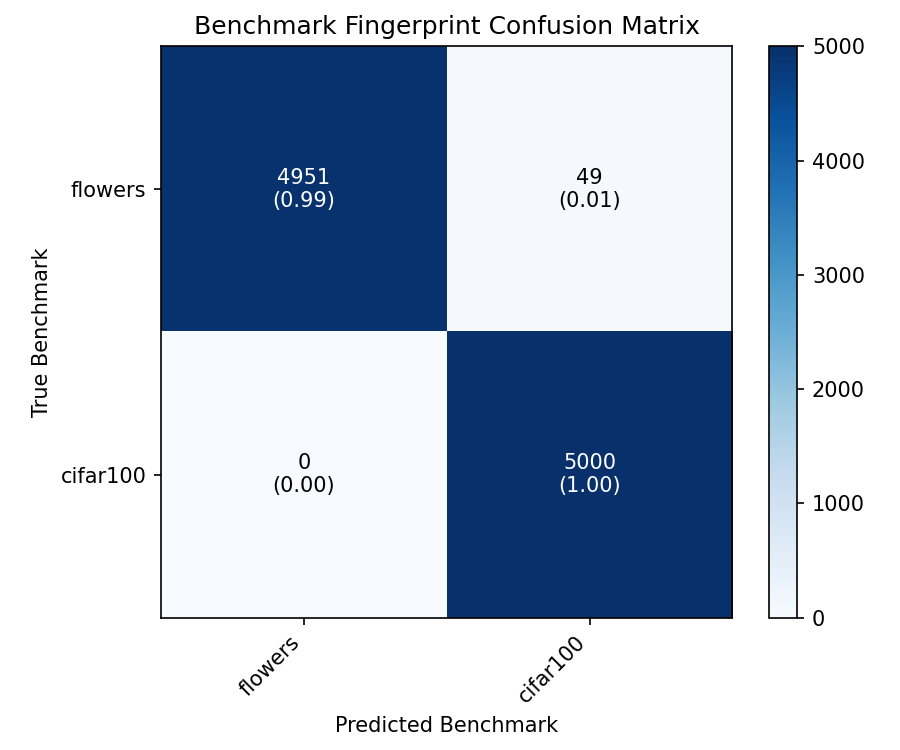
\includegraphics[width=\columnwidth]{figures/confusion_matrix.png}
\caption{Confusion matrix for benchmark fingerprint classification}
\label{fig:confusion_matrix}
\end{figure}

\textbf{Figure 1:} Confusion matrix for benchmark fingerprint classification (H-E1). The classifier achieves 99.51\% accuracy with asymmetric errors: CIFAR-100 representations are never misclassified, while 49/5000 (0.98\%) Flowers102 samples are incorrectly classified as CIFAR-100.

\begin{figure}[htbp]
\centering
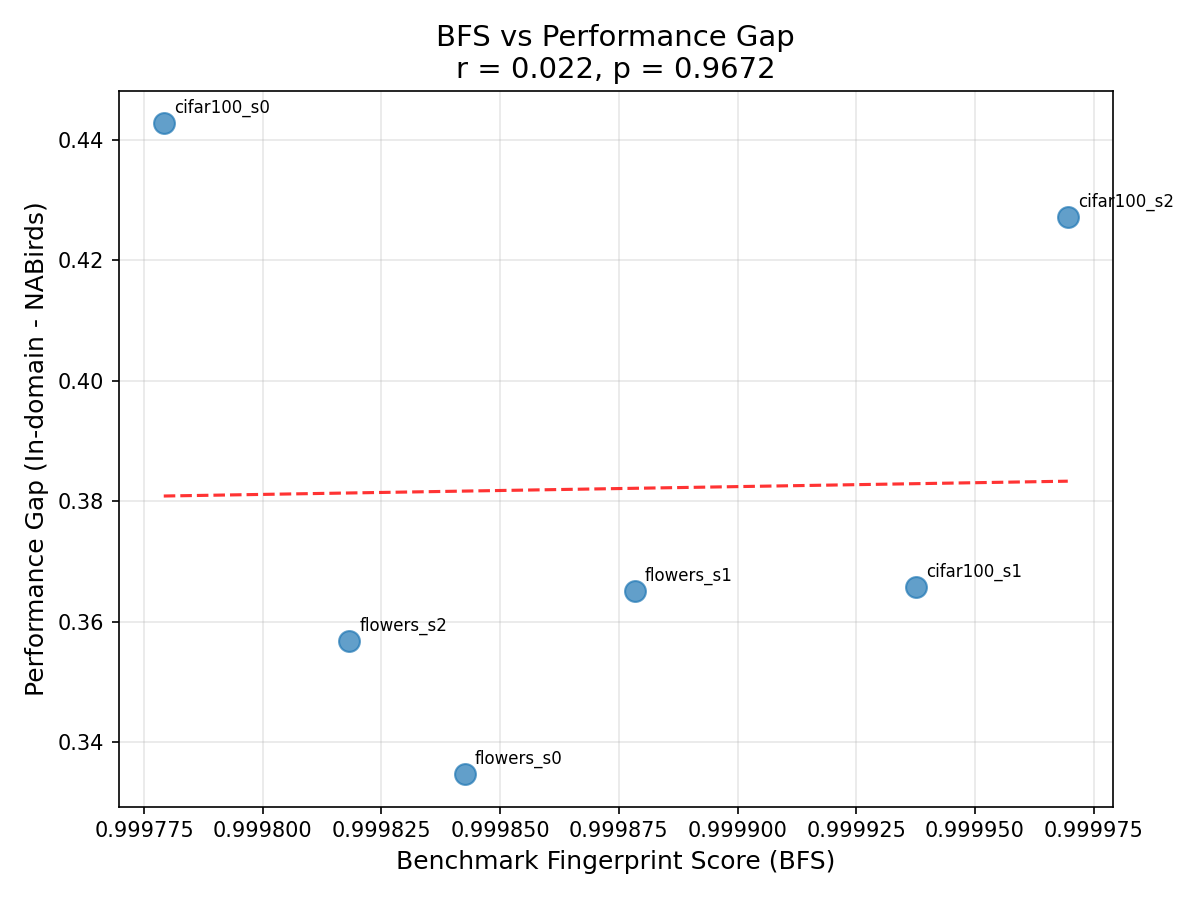
\includegraphics[width=\columnwidth]{figures/bfs_gap_scatter.png}
\caption{BFS vs. cross-dataset gap scatter plot}
\label{fig:bfs_gap_scatter}
\end{figure}

\textbf{Figure 2:} BFS vs. cross-dataset gap scatter plot (H-M1). No correlation is observed (r = 0.022, p = 0.967). All models cluster at BFS > 0.999, demonstrating the ceiling effect that prevents correlation analysis. Gap values range from 33.5 to 44.3 percentage points.
